\documentclass[conference,a4paper,twoside]{IEEEtran}
\usepackage[utf8x]{inputenc}
\usepackage{ucs}
\usepackage{amsmath}
\usepackage{amsfonts}
\usepackage{amssymb}
\usepackage{graphicx}
\author{Daniel Thomas}
\begin{document}
\title{Security of deployed Android devices}


% author names and affiliations
% use a multiple column layout for up to three different
% affiliations
\author{
\IEEEauthorblockN{Daniel Wagner,
Daniel R.\ Thomas,
Alastair R.\ Beresford,
Andrew Rice}
\IEEEauthorblockA{
Computer Laboratory\\
University of Cambridge\\
Cambridge, United Kingdom\\
Firstname.Lastname@cl.cam.ac.uk
}
}


\maketitle


\begin{abstract}
Android is the most popular smartphone platform and seeks to provide better security than popular desktop operating systems through increased compartmentalisation and a permission system for apps.
This security relies on there not being root privilege exploits which allow apps to bypass all protections.
Many such exploits have been found and fixed.
Our hypothesis is that these fixes do not promptly reach the users devices and so much of the time users are running versions of Android known to be vulnerable.
We used the DeviceAnalyzer data\cite{TODO} and found that over XX\% of devices were exposed to known vulnerabilities on average. %TODO (drt24) proportion of devices exposed on average.
There was also a period of several months when no devices ran secure versions of Android.
\end{abstract}

\section{Introduction}
Android has XX\% of the smartphone market~\cite{TODO} and while the core development is controlled by Google there are at least XX~\cite{TODO} manufacturers which make devices which run Android.
Many of these manufacturers customise the version of Android they ship and sometimes network operators (of which there are at least XX~\cite{TODO}) make further modifications.
Hence when Google produces an update to Android, the update may have to pass through the manufacturer and operator before reaching the user.
The manufacturer and user have no financial incentive to perform this work.
There is ongoing legal action to force some of them to do so~\cite{TODO}.

Android relies on the Linux kernel to provide compartmentalisation and runs each app as a separate unix `user'.
The Linux kernel is a large piece of software and so there will always be new root exploits found in it~\cite{TODO}.
Manufacturers of Android devices have also added further root exploits when customising it~\cite{TODO}.
Between XX\%~\cite{TODO} and XX\%~\cite{TODO} of malware for Android contains root exploits.
While this shows that much Android malware does not need a root exploit to work, it can just request the relevant permissions and the user will grant them, a significant proportion does.
This malware is also more dangerous because while ordinary malware can be remotely removed by Google through the Play store, once a root exploit has been used there are no guarantees.

Figure \ref{fig:proportioninsecure} shows the proportion of Android devices in the DeviceAnalyzer data which were running versions of Android known to root exploits at the time.


\begin{figure}[!b]
\centering
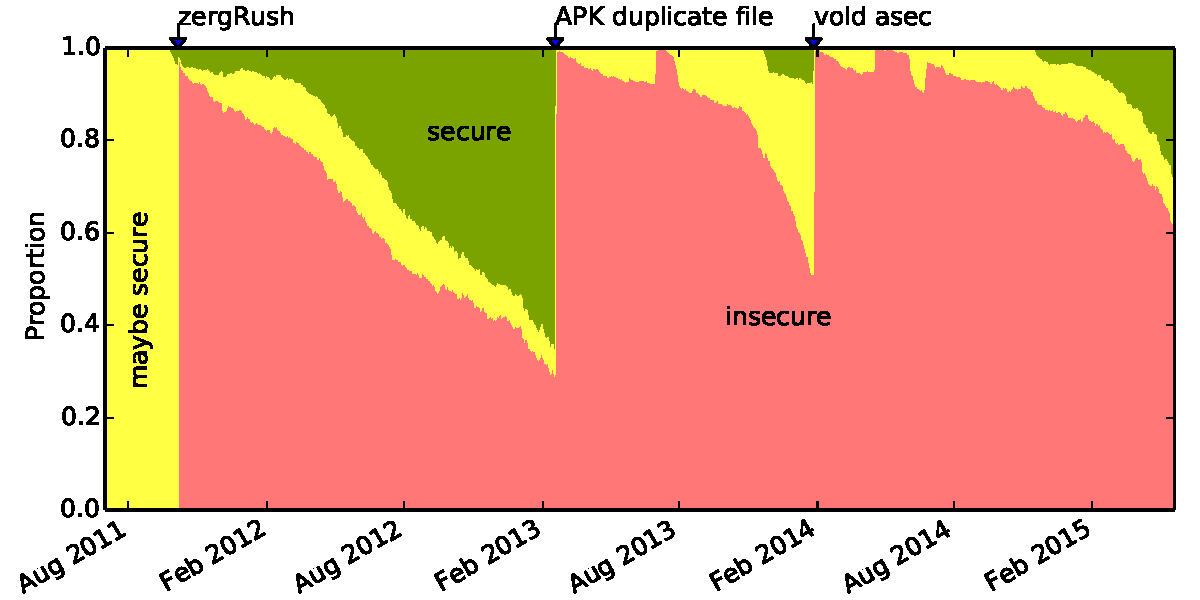
\includegraphics[width=\columnwidth]{figures/proportioninsecure}
\caption{Proportion of devices running insecure versions of android}
\label{fig:proportioninsecure}
\end{figure}

\section{Background}

\section{Results}

\section{Related work}
Stopping root exploits working: SEAndroid.
Detecting malware: Android antivirus useless.

\section{Conclusion}

\end{document}